\documentclass[letterpaper]{sig-alternate}
\usepackage{amsmath}
\usepackage{amssymb}
\usepackage{listings}
\usepackage{courier}
\usepackage{multirow}

% Include PDF graphics, configure our images directory, and specify image types.
\usepackage{graphicx}
\usepackage{epsfig}
\graphicspath{{./images/}}
%\DeclareGraphicsExtensions{.pdf,.jpeg,.png,.jpg}
\DeclareGraphicsExtensions{.eps}

% Style listings
\lstset{%rulesepcolor=\color{Gray},
        frame=single,                        	% Shadow box frame around code
        basicstyle=\scriptsize\ttfamily,        % Use small true type font
        showstringspaces=false,                 % Don't put marks in string spaces
        morecomment=[l][\color{Blue}]{...},     % Line continuation (...) like blue comment
}

\begin{document}

\title{A Domain Specific Language for Usage Management}

\numberofauthors{1}

\author{
\alignauthor
Christopher C. Lamb, Pramod A. Jamkhedkar, Mathew P. Bohnsack, Viswanath Nandina, Gregory L. Heileman \\
       \affaddr{University of New Mexico}\\
       \affaddr{Department of Electrical and Computer Engineering}\\
       \affaddr{Albuquerque, NM 87131-0001}\\
       \email{\{cclamb, pramod54, mbohnsack, vishu, heileman\}@ece.unm.edu}
}

\conferenceinfo{DRM'11,} {October 21, 2011, Chicago, Illinois, USA.} 
\CopyrightYear{2011} 
\crdata{978-1-4503-1005-5/11/10} 
\clubpenalty=10000 
\widowpenalty = 10000

\maketitle

\begin{abstract}
In this paper we describe the development of a domain specific language (DSL) for expressing usage management policies and associating those policies with managed artifacts.  We begin by framing a model for the language, including generalized use cases, a domain model, a general supported life-cycle, and specific extension requirements.  We then develop the language from that model, demonstrating key syntactic elements and highlighting the technology behind the language while tracing features back to the initial model.  We then demonstrate how the DSL supports common usage management and DRM-centric environments, including creative commons, the extensible rights markup language (XrML), and the open digital rights language (ODRL).
\end{abstract}

\category{D.3.0}{Software}{Programming Languages}[General]
\terms{Design, Languages, Security}
\keywords{Access Control, Interoperability, DRM, Usage Management}

\section{Introduction}
In this paper, we define usage management as the ability to control actions over resources and data across and within computing environments.  More than access control or digital rights management, usage management addresses with fine-grained control of all aspects of how a given digital resource is used.  As digital environments become more open over time, the need for usage management for resources that span utility computational environments (e.g. cloud provider systems) will become increasingly important \cite{ctrl:lamb-MCCCS,ctrl:lamb-SOSE}.

With the advent and widespread use of cloud computing, those responsible for a given usage managed resource are almost never those responsible for the computing systems, except at edge devices like mobile phones or other small profile computing devices.  Resources are regularly moved across national boundaries and regional areas without either the content owner's or creator's knowledge.  Furthermore, this kind of transfer is generally according to pre-established algorithms or data routing protocols over which users have no control.  Managing these issues requires new usage management capabilities that can run on platforms ranging from small, hand-held devices to nodes in large data centers.

Research in this area has been focused on developing more expressive policy languages via either different types of mathematical logics or formalisms with greater reasoning capabilities~\cite{ArHu:07,BaMi:06,ChCoEtHaJoLa:03,HaWe:04,HaWe:08,PuWe:02,XiBjFu:08}.  These approaches however fail to address interoperability challenges posed by new commercially available distributed computing environments.  Interoperability efforts have resorted to translation mechanisms, where the policy is translated in its entirety to a different language~\cite{HeJa:05,PoPrDe:04,ScTaWo:04}; it has been shown recently however that such techniques are infeasible and hard to perform for most policy languages~\cite{KoLaMaMi:04, SaShUe:04}. Other approaches have led to complex policy specification languages that have tried to establish themselves as the universal standard~\cite{OMADRM,ODRL-req,Wa:04,XrML-spec}.  This unfortunately tends to stifle both innovation and flexibility~\cite{HeJa:05,JaHe:04,JaHe:08,JaHeMa:06}.

To address these issues, we first applied the principles of system design to develop a framework for usage management in open, distributed environments that supports interoperability. These principles have been used by researchers in large network design to create a balance between interoperability and open, flexible architectures~\cite{Al:04,BlCl:01,ClWrSoBr:02}, without sacrificing innovation. Initially we standardized certain features of the framework operational semantics, and left free of standards features that necessitate choice and innovation.

We have implemented this framework, including a usage management calculus providing a platform for usage management, within a Domain Specific Language (DSL) and associated evaluation environment. The DSL and its environment implements the previously defined framework, separating various roles needed for distributed policy creation and management, provides the capability to develop executable licenses, and is extensible from both a policy and constraint definition perspective.

In this paper, we will first review the problems in usage management in more detail, providing the context for this DSL and the problems it helps solve.  Then, in Section \ref{sec:model} we will first review the model we developed to guide the DSL's syntactic and semantic development. In the next section, we will cover the language itself, how it was developed, and its supporting evaluation environment.  We will then close the paper with three specific implementation examples showing how the language and its runtime support usage management scenarios from three different environments --- creative commons (CC), the extensible rights markup language (XRML), and the open digital rights language (ODRL).

\section{Motivation}\label{sec:motivation}
Usage management incorporates specific characteristics of traditional access control and digital rights management incorporating encryption mechanisms, trust management, and trusted computing platforms \cite{Jamkhedkar:2010:IUM:1866870.1866885}.  In order to be effective, it must be flexible enough to provide users with opportunities for differentiation and extension, but inter-operable enough to provide services across widely diverging computational environments.

This DSL and runtime provide flexibility through the inclusion of easily pluggable constraint and policy evaluators.  Both types of evaluators simply need to be locatable by the runtime, via standard classpath-style semantics.  If they are, they can be loaded and used with no other configuration required.  A policy file can simply reference the evaluator via a predefined language element, and the runtime will find it and load it automatically, using it to evaluate either the policy itself or the defined constraints (depending on whichever type of evaluator is specified).

The policy runtime elements can be dynamically loaded on host systems when required.  This provides interoperability by forcing the policy system itself to accept the responsibility of ensuring it is installed wherever needed.  The technology upon which the runtime is based is widely available as well.  Additionally, the policies can be transferred from one host to another and can be directly executed upon delivery.  Furthermore, this language and system can express the semantics of common rights management environments, providing additional semantic flexibility and interoperability.

The DSL we describe, in tandem with its runtime, embodies an inter-operable framework for usage management, unlike Coral and Marlin architectures, that implements a formal calculus to reason about the relationship between a license, a computing environment, and interoperability between them. It incorporates concepts such as programmable licenses and common ecosystems used by Coral and Marlin architectures respectively. The DSL design is based on the principles of {\em design for choice}, eloquently described by Clarke et al. with reference to ``tussles'' in cyberspace~\cite{ClWrSoBr:02}. They explain the importance of identifying the locations in the architecture where standards need to be introduced to enable interoperability, and locations where they should {\em not} be applied to enable innovation and differentiation.  By supporting pluggable evaluators that allow users to extend the basic language syntax, semantics, and runtime arbitrarily, this language system provides space for innovation.

\section{Language Model}\label{sec:model}
In developing this DSL, we needed to have a clear understanding of the specific domain, and develop and appropriate domain model to guide our efforts.  Admittedly, there exist many possible models that can describe this area of policy and policy management, and the model that we chose to initially use is purposefully simple to help ease development and implementation efforts.  We did however provide arbitrary language-level extensibility to support future extension into more demanding policy implementation areas.

\begin{figure}[!t]
\centering
\includegraphics[width=2.5in]{blank}
\caption{Conceptual Model}
\label{fig:model:conceptual-model}
\end{figure}

Our expectation, reflected in Figure \ref{fig:model:conceptual-model}, is that we have created a system through which three primary actors work in tandem to create executable policies that can be converted into licenses in order to manage the use of defined content.  The process starts with a context designer, who specifies the environment in which a resource can be used by a specified subject.  This context is then applied by a policy designer to create specific policy language, which is then used by a policy author to create a policy.  The policy itself is manipulated behind a defined interface that requires an instantiation of the defined context from a usage management system.

We developed this model to help us understand how policy-centric DSLs would be used, to visualize how the various elements are inter-related, and to clarify important areas upon which to focus effort.  Through this model, we were able to conceptualize the initial language structure and generate performance hierarchies, as well as to tailor expected DSL use.

\subsection{Expected Use}
In order to develop the appropriate DSL giving users the power and expressivity they need to easily express usage management concepts, we begin by developing a model describing how we expect it to be used, and by whom, identifying key functional and non-functional characteristics.  We use roles codified as actors to identify the primary user base, and link those roles to specific use cases we expect to be common in day to day DSL use.  We also identify common inputs and outputs from expected activities, and show how those input and output elements are related.  We finally specify the essential core structure of the DSL, as well as extension points and default implementations of those points.

In general day to day use, we expect that certain activities will be much more common that others.  For example, each \textit{policy} requires a \textit{context} in order to both be developed and to run.  That \textit{context} describes the actors using an artifact protected by a policy, the artifact itself, and the environment in which the artifact is both expected to be used (during policy design) and is being used (at evaluation).  That said, the expectation is that the number of policies is much greater than the number of contexts associated with those policies.

Likewise, we expect that the number of times a policy is evaluated is much greater than the number of times that policy is designed and created.  Policies should be read, evaluated, or combined with other policies frequently.  This gives us a magnitude ordering for these activities, where the number of supported contexts is much less than the number of created policies, which is in turn much less than the number of times that policy is evaluated or otherwise used.

This has specific implications on both the DSL syntax and performance profile.  For example, as it is much more common for policies to be evaluated than contexts to be created, our efforts and tuning the system and increasing performance are best focused on policy evaluation rather than contextual activities.  In a similar vein, the language itself should be as simple to comprehend as possible for policies at the expense of contextual elements if necessary.

\begin{figure}[!t]
\centering
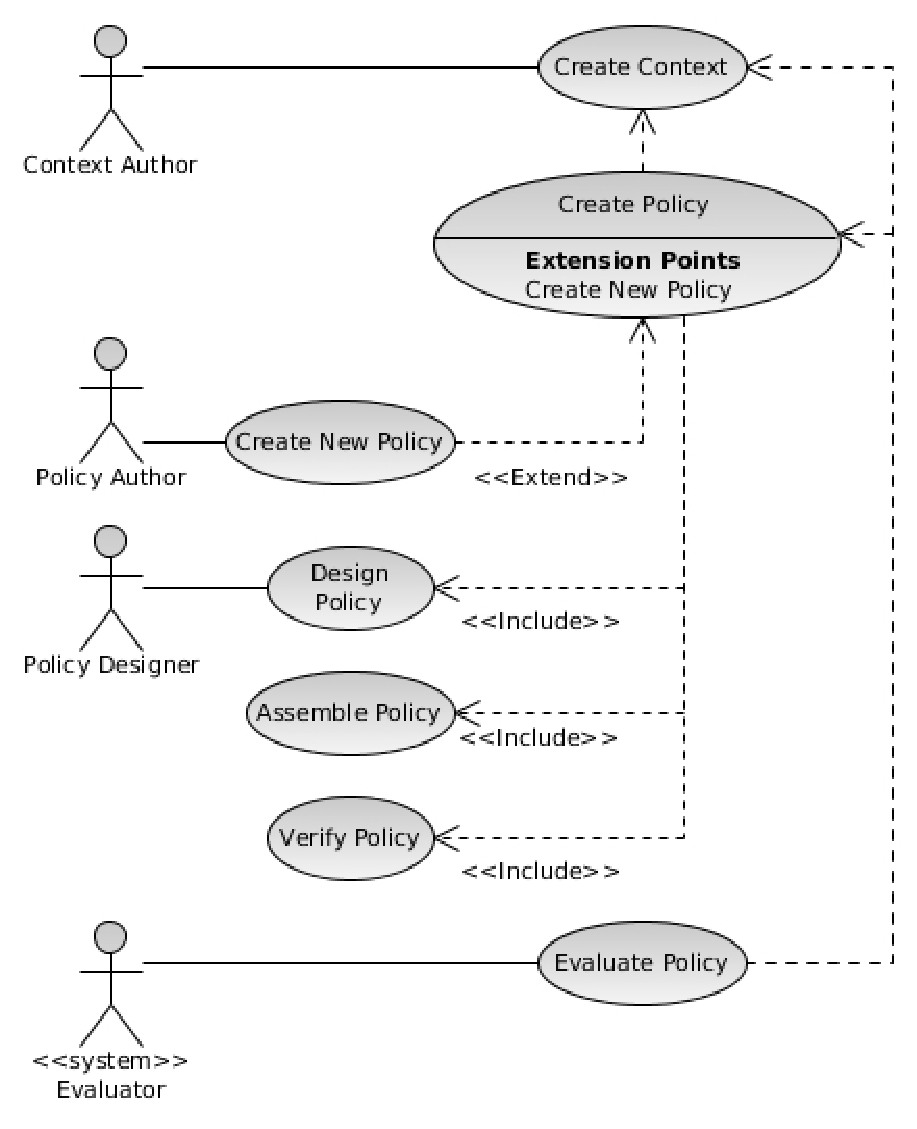
\includegraphics[width=3in]{use-cases}
\caption{General DSL Use Cases}
\label{fig:model:use-cases}
\end{figure}

Figure \ref{fig:model:use-cases} shows the primary system actors we have identified as well as the use cases with which they will be involved.  Actors include:
\begin{itemize}
\item \textit{Context Author}.  The context author is responsible for defining the context in which a policy will be applied to a given resource.  The context itself defines the environment in which the policy executes, the resource to which the policy is applied, and the subject that attempts to use the resource.
\item \textit{Policy Designer}.  The policy designer is responsible for putting together a specification for a given policy that a policy author can use to build an instance of a policy.  The person in this role is also responsible for building various policy evaluation components for the DSL if needed.  
\item \textit{Policy Author}.  The policy author creates a policy to control the use of a subject defined in the policy context.
\item \textit{Evaluator}. Another system element, an evaluator evaluates a given policy with a specific context.
\end{itemize}

When a context author creates a context, that author compiles the elements of that context for use both at policy creation and policy execution.  When the policy is initially created, the resource is the only defined element.  Generally both the subject, representing the eventual user, and the environment, containing information describing the evaluation environment, are only defined at the classifier level.  That is to say, they both are defined, but individual properties have yet to be assigned.

Creating a policy is an activity undertaken by a policy author.  This step requires a \textit{declared} (but not \textit{defined}) context.  This is also undertaken in tandem with some kind of policy specification that describes roughly what the policy should manage and how it should be managed.  In the ontology we have defined, this is the step at which the policy designer defines the various constraints, activities, restricted activities, and obligations and develops the appropriate DSL components required to evaluate that policy.  Creating a new policy is precisely what it describes - creating a brand new policy applied to a context.

The included cases define policy, assemble policy, and verify policy are common development steps through which the policy is essentially designed, developed, and then tested against a context.

Finally, a policy is evaluated by an evaluator, a system actor, after creation and association with a resource.  At this point, the context has a fully instantiated context, with defined resource, subject, and environmental elements.

Now we have a general understanding of the expected use of a given policy, and have defined the expected roles.  With this in place, we begin to look at the elements the DSL should have to allow it to express the use cases we expect we need to support as the next step in refining our understanding of what this DSL should look like.

\subsection{Domain Model}
Our domain model will be the foundation of our DSL.  It will allow us to begin to understand the various language elements and how they are related, leading us to an eventual syntax to represent these classifiers and relationships.  Not understanding this structure well, or developing a structure that does not support our defined use cases will lead us to develop a DSL that inadequately supports our expected use.

Based on our use cases, we know the model contains a \textit{context}, some kind of policy-specific sub-ontology, and a logic engine that can act over that sub-ontology.  Based on our current understanding of our needs, the sub-ontology contains \textit{obligations} and \textit{constraints} applied to \textit{activities}.  We use simple first-order logic to reason over the policy elements.

This understanding leads us to the model view in Figure \ref{fig:model:ontology}.  Of special note, the specific policy sub-ontology is contained in the usage semantics package, as is all policy evaluators.  Both of these can change within this model to allow for inclusion of more complex policy systems and powerful reasoning capabilities.

Primary elements within this ontology are:
\begin{itemize}
\item \textit{Runtime}.  This is the system that manages use of a given \textit{resource} by a \textit{subject} in accordance with a \textit{policy}.  It is responsible for providing and managing context elements, controlling policies and licenses, and handling requests from subjects.  Realizations of this system must be cross platform to support distributed use as well.
\item \textit{Context}.  The context describes the operating environment of the policy.  This information must be available at runtime, and parts of it must be understood when the policy is initially designed.  In order to effectively control use of a given artifact, the parameters that artifact can be used under must be understood when the policy is created and must be read when that policy is evaluated.
\begin{itemize}
\item \textit{Environment}.  The environment in which a given policy is evaluated.  This must be understood in order to constrain the conditions where a policy will allow or disallow artifact access.  This is essentially an associative array, where the keys are specific expected properties of a given environment.
\item \textit{Resource}.  A resource is the artifact over which the policy controls use.  This can be any type of artifact whatsoever, ranging from documents to media files to streaming data.  A resource may also have arbitrary properties like an associated URI, a canonical name, a MIME type, or creation metadata.
\item \textit{Subject}.  Subjects use a given resource.  Acceptable use is described by the policy.
\end{itemize}
\item \textit{Policy}.  A policy describes the conditions of use for a given resource.  In our example, this includes information on acceptable contexts and subjects, as well as obligations and constraints.  Policies can be configured in this DSL to use arbitrary evaluators.  This allows users to implement specific policy semantics tailored to their domain if needed, though they are free to use packaged syntax evaluators if those evaluators fit their needs. 
\item \textit{Usage Semantics}.  As policies can implement arbitrary semantics, they can be based on an specific models tailored to the needs for the particular policy system.  For example, this DSL currently implements obligations and constraints restricting defined activities.  Other domains may need to use more descriptive semantics, perhaps addressing causality or ordering.
\end{itemize}

\begin{figure}[!t]
\centering
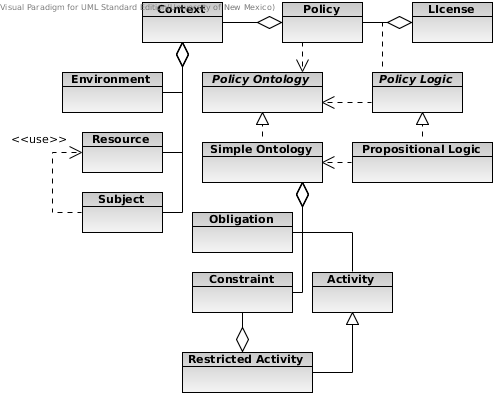
\includegraphics[width=2.5in]{ontology}
\caption{Basic Language Model}
\label{fig:model:ontology}
\end{figure}

Current usage semantics package various evaluators (specifically constraint and policy evaluators) and related entities as shown in Figure \ref{fig:model:usage-semantics}. Flexibility in policy evaluation is provided by pluggable \textit{evaluators}.  These evaluators essentially execute a given policy in tandem with a supplied context.

\begin{itemize}
\item \textit{Evaluators}.  Evaluators are pluggable components that provide flexibility in policy capability.  We currently use two --- one for evaluating policies, and one for evaluating constraints.  Policy designers can also specify multiple evaluators to enable combinations of semantics, as long as those semantics are not in conflict.  Evaluators can use any kind of computational model or logic as well.  For example, one evaluator may use a simple state machine model to evaluate a policy, while another may use a more complex turing-complete model.
\begin{itemize}
\item \textit{Policy Evaluator}.  This evaluator is responsible for evaluating the policy as a whole.  To do so, it evaluates the relationships between permissions and obligations, and uses the constraint evaluator to examine restricted activities.
\item \textit{Constraint Evaluator}.  Constraint evalutators specifically examine constraints defined within restricted activities.  They can do so using arbitrary evaluation rules ranging from simple conjunctive evaluation (where all constraints must be true) to more complex schemes where, for example, a certain number of constraints must be true while one of a set of other constraints must be false.
\end{itemize}
\item \textit{Obligation}.  An obligation describes a restricted activity that must have occurred or must occur in the future for a restricted activity to be performed.  For example, a media stream may wish to obligate users to purchase access to that stream on the third access.
\item \textit{Permission}.  In this context, a permission is a restricted activity that a subject can perform under the condition that certain specified obligations are met.
\item \textit{Constraint}.  A constraint generally constrains a restricted activity.  This could be as simple as limiting use to a single identifiable subject or as complex as limiting use based on time and date, user identity, and geographic location.
\item \textit{Activity}.  A general activity is something a subject would wish to do in association with an artifact.  It describes how a \textit{subject} would use a \textit{resource} in an unrestricted way, or some action that \textit{subject} performs.
\item \textit{Restricted Activity}.  When an activity is embellished with constraints or obligation, it becomes restricted.
\end{itemize}

Now we have rigorously defined the domain elements our DSL will address.  Keep in mind, this domain model allows us to dynamically replace ontology elements in that all \textit{policy ontology} and \textit{policy logic} elements can be replaced on per-policy basis.  This would allow us to create multiple policies described using disparate ontologies and related evaluation logics if needed to more fully describe restrictions in a specific evaluation domain.

We have also separated the definition of \textit{activities} from \textit{restricted activities}.  This separation of concerns allows policy developers to define a single activity which can then be reused across a large number of restricted activities based on specific varying constraints.  For example, if I have a write activity, I can constrain that activity in slightly different ways to create a relatively large number of related restricted activities.  I could restrict write by geographic area, by subject identification, by date and time, or by having contributed to some political cause, creating four restricted activities from the same base activity.

The base domain model however, based on contextual elements, policies, and licenses does not change.  This stability allows for ease of runtime integration as it hides any policy evaluation-specific changes.  As long as a given logic and policy ontology is delivered with a given policy, the policy evaluation runtime will be able to evaluate that policy against resources and subjects in a given environment.  In essense, this is a layered model where the context and policy elements compose the user interoperability layer while policies and policy logics form a more dynamic policy expression layer.  This way, resource users have a stable runtime view of policies and policy managed resources, while policy and context developers have the flexibility to implement policies at arbitrary levels of expressibility.

\begin{figure}[!t]
\centering
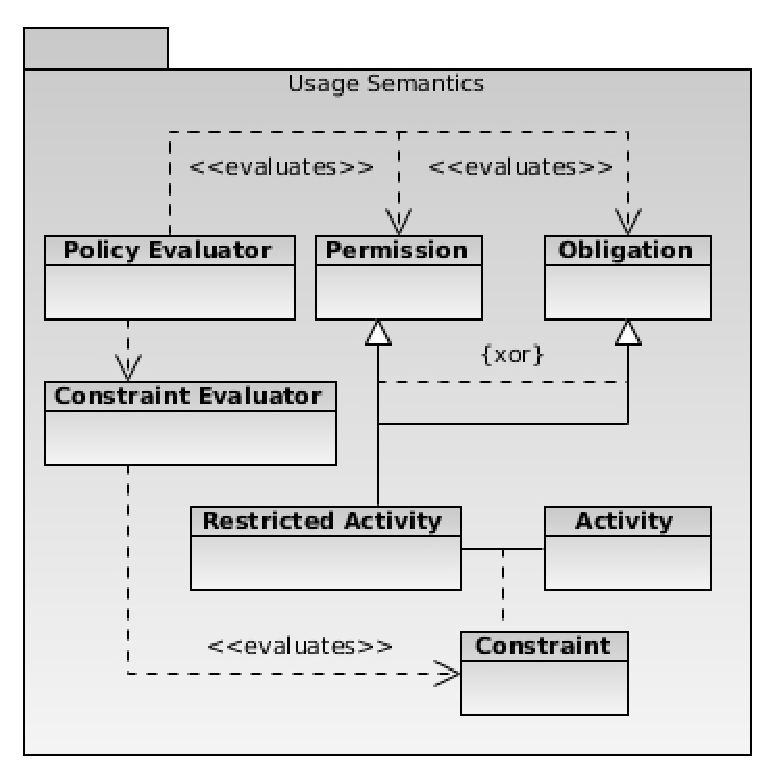
\includegraphics[width=2.5in]{usage-semantics}
\caption{Current Usage Semantics}
\label{fig:model:usage-semantics}
\end{figure}

\subsection{Envisioned Lifecycle}

\begin{figure}[!t]
\centering
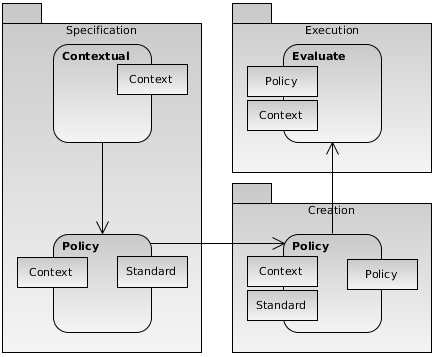
\includegraphics[width=3in]{lifecycle}
\caption{Policy Development Lifecycle}
\label{fig:model:lifecycle}
\end{figure}

\subsection{Language Components}

\begin{figure}[!t]
\centering
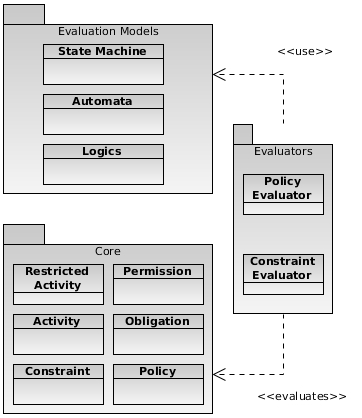
\includegraphics[width=2.5in]{language-components}
\caption{Language Elements}
\label{fig:model:language-components}
\end{figure}

\section{Language}\label{sec:language}


%\begin{figure}[!t]
%\centering
%\includegraphics[width=3in]{cloud-current}
%\caption{Single SLA with Control Elements}
%\label{fig:current-cloud-model}
%\end{figure}
\section{Applied}\label{sec:applied}
Now that the DSL has been modeled and implemented, we can apply it to a variety of common usage management domains.  In order to demonstrate the DSL's power and flexibility, we have chosen to implement examples from creative commons, the open digital rights language, and the extensible rights markup language.

\subsection{Creative Commons}\label{sec:model-cc}
In this section, we use our DSL to implement a policy that can be used with creative commons licensed content.  The creative commons is a nonprofit organization that provides free, easy-to-use legal tools that provide a simple, standardized way to pre-clear usage rights to creative works for copyright owners.  It gives copyright holders an easy way to license their works in a way that leaves ``some rights reserved'' as compared to the ``all rights reserved'' default.  By providing these legal tools, the creative commons hopes to increase the amount of creativity available ``in the commons'' \cite{creative-commons}.

Seven main license types are defined by creative commons:

\begin{itemize}
\item \textbf{Public Domain}. This license does not put any restrictions on how others may remix, tweak, or build upon your work.
\item \textbf{Attribution}.  This license lets others distribute, remix, tweak, and build upon your work, even commercially, as long as they credit you for the original creation. This is the most accommodating of the licenses offered.  It is recommended for maximum dissemination and use of licensed materials.
\item \textbf{Attribution, Share-Alike}.  This license lets others remix, tweak, and build upon your work even for commercial purposes, as long as they credit you and license their new creations under the identical terms.  This license is often compared to free and open source software licenses.  All new works based on yours will carry the same license, so any derivatives will also allow commercial use.
\item \textbf{Attribution, No-Derivatives}.  This license allows for redistribution, commercial and non-commercial, as long as it is passed along unchanged and in whole, with credit to you.
\item \textbf{Attribution, Non-Commercial}.  This license lets others remix, tweak, and build upon your work non-commercially, and although their new works must also acknowledge you and be non-commercial, they do not have to license their derivative works on the same terms.
\item \textbf{Attribution, Non-Commercial, Share-Alike}.  This license lets others remix, tweak, and build upon your work non-commercially, as long as they credit you and license their new creations under identical terms.
\item \textbf{Attribution, Non-Commercial, No-Derivatives}.  This license is the most restrictive of the licenses, only allowing others to download your works and share them with others as long as they credit you, but they cannot change them in any way or use them commercially.
\end{itemize}

Now that we have explained the different creative commons license types, what they mean, and the restrictions they have, we will create a policy with our DSL that represents compliant usage of creative commons licensed works.

First, we use our DSL to define an activity.  In creative commons there is really only one activity ---  sharing a creative commons licensed work --- so this code is fairly simple, defining the \texttt{share} activity.

\lstinputlisting[]{content/code/cc/activity.rb}

Next, we define constraints on the \texttt{share} activity.  There are four such constraints in creative commons, as discussed above: attribution, commercial use, derivative work, and share-alike.  This results in four constraints defined in our DSL:

\lstinputlisting[]{content/code/cc/constraints.rb}

Finally, we define the restricted activities, covering all seven basic license types.  For example, in the following code listing, the \texttt{share\_by\_work} restricted activity is defined by associating the \texttt{attribution} constraint with the \texttt{share} activity. Likewise, the \texttt{share\_by\_sa\_work} restricted activity associates the \texttt{attribution} and \texttt{share\_alike} constraints with the \texttt{share} activity.  Sharing activites for all seven license types are defined similarly, resulting in a policy that allows for sharing all types of Creative Commons licensed works, with proper constraints.

\lstinputlisting[]{content/code/cc/restrictedactivities.rb}

Now that we have implemented basic policy protections as defined in the creative commons environment, we will move on to ODRL.
\subsection{ODRL}\label{sec:model-odrl}
ODRL provides the necessary semantics for Digital Rights Management expressions in an open and trusted environment. By analyzing the ODRL language we can show that it can be mapped to the framework. In the ODRL Expression language there are different models.  Specifically, we are going to demonstrate how ODRL-centric permissions, constraints, requirements, and conditions can be expressed in the DSL.

In ODRL, \emph{permissions} are related to \emph{actions} that a \emph{subject} can execute on a \emph{resource} of some kind and generally encapsulate use, reuse, transfers, and general asset management.  The following analysis is modeled on ORDL v. 1.1 \cite{Ia:02}.

In the DSL we limit \emph{activities} with \emph{constraints}. Limiting an activity with a constraint yields a \emph{restricted activity}. This restricted activity can be either an obligation or a permission. While evaluating these permissions, necessary steps must be taken to maintain the restrictions. On the other hand, in ODRL constraints are directly associated with the permissions rather than actions.  Furthermore, constraints in this DSL are more flexible than those in ODRL generally. While ODRL constraints have two operands and a single operator, and are conjunctively evaluated, constraints in this DSL can be any kind of predicate with an arbitrary argument list and extensible semantics.

In ODRL, the condition model holds that if any condition is satisfied, indicating that an event did occur, then related permission is not granted. In the framework outlined in this paper, we can express this either with specific constraints or via obligations.  Constraints would generally involve the current execution context in which the policy is evaluated, and would render a usage decision based on that information.  Obligations are essentially activities, and can be activities that should have been performed prior to use, and as such can model conditions as well.

The last part is the context model. If we take into account the context model in ODRL, each and every entity has its own independent context whereas in the DSL all the entities lie inside a common context.  This allows for ease of ontology sharing between the various components operating within a given context.

To demonstrate the mapping between the ODRL model and the framework, we will examine a scenario and express it as an ODRL license and then create an equivalent DSL. Consider a scenario where a user wants to listen to music from an on-line music library. To get access to the library the user has to pay the amount of \$15 USD. The music file can only be played on a windows based device within United States.

\lstinputlisting[]{content/code/odrl/odrl.xml}

\vfill\eject
The equivalent DSL would be:

\lstinputlisting[]{content/code/policy/example.pol}

In the DSL, the first activity is \emph{listen}, bounded by the constraint {\em c1} that the user can listen to the music only within United States and that the device must be a windows device. When constraints are applied to the first activity it is then called restricted activity {\em ra1}. Similar constraints are reflected in the ODRL snippet.

The second activity is \emph{payment}, bounded by a constraint {\em c2} that the user needs to pay an amount of \$15 USD to get access to the music file. We then call this activity as restricted activity {\em ra2} after the constraint {\em c2} is applied. 

Then we define a policy which allows permission to the first restricted activity {\em ra1} when second restricted activity {\em ra2} is true. So, {\em ra2} is an obligation that needs to be fulfilled in order to get permission for {\em ra1}. This obligation is represented as a requirement in ODRL.

This example demonstrates clear equivalence in this particular domain.  The extensible nature of the DSL's evaluators could provide any missing functionality in more detailed cases as well, but in general, any problem representable in ODRL is also representable within this DSL.
\subsection{XRML}\label{sec:model-xrml}
Extensible Rights Markup Language (XrML) is a language used to define a user's rights over a resource of some kind. It helps the owner of a digital resource to identify the users allowed to access that resource, what rights are available to those users, and the conditions under which those rights may be applied. Here, we are interested in mapping the grant, principal, right, resource and condition concepts into our framework \cite{XrML-spec}.

A \emph{principal}, in XrML, is someone who has been granted \emph{rights} to a specific \emph{resource}.  In this context, \emph{grant} refers to the act of giving or temporarily providing those resource rights.  A \emph{right}, associated with a \emph{grant}, is some kind of action the principal can perform on a given resource, like listening to a song or editing a video stream.  \emph{Conditions} specify specific terms under which a principal can wield rights over a resource.

In this DSL, the principal is a subject, grant is permission and right an activity. A resource in XrML is the same as resource in our DSL's implementation. The concept of condition in XRML maps to our obligations and constraints.

Using the same scenario we used in the ODRL example, we have build a representative XrML file describing user rights in this particular context:

\lstinputlisting[]{content/code/xrml/xrml.xml}

In this XrML license, the principal is the user who wants access to the music library. The rights holder gives the right to listen to a resource given the condition that the country in which the the listening occurs is the United States and the device is windows based. Furthermore, the principal must also have already made a payment of the amount USD \$15.  In the DSL fragment from the previous section, payment and listen are defined as activities, whereas listening to music only on windows based devices and within United States is a constraint. When the above constraints are satisfied the user then has permission to access the resource.

\section{Conclusions and Future Works}
Usage management is a common problem set with features embodied in domains ranging from security systems to video games to music production and retail.  The ability to provide management of resources with regard to authorized subjects is being addressed in multiple different forums, many of which are taking remarkably different approaches.  Common features however generally include the need for either ubiquitous rights expression language acceptance or for extensive translation between all supported rights languages.

In this paper, we first demonstrated the development of the initial model we used to define our problem space.  Here, we described the general use of the system, who the primary users were, what the expected lifecyle of policies was, and what the domain model looked like.  We then implemented the syntax of the DSL, in Ruby, as an internal DSL with specific examples.  We wrapped up the paper with demonstrations of equivalence to common rights management frameworks like the creative commons, ODRL, and XrML.

We have only begun to specify and use this particular DSL.  Future focus for our group on this effort will include additional language elaboration, exploration, and use in specific scenarios.  We need to spend additional time engineering the underlying software as well, so we can ensure that policies are in fact platform and environment agnostic, portable, and executable.  Finally, this implementation is an internal DSL within the Ruby language; we need to explore the application of external DSL techniques to this domain to better understand the required compromises between expressiveness and development difficulty and begin to apply more stringent security models to the system itself.

\begin{thebibliography}{10}

\bibitem{OMADRM}
Enabler release definition for {DRM} {V}2.0.
\newblock Technical report, Open Mobile Alliance, 2003.
\newblock {\small
  \verb%xml.coverpages.org/OMA-ERELD_DRM-V2_0_0-20040401-D.pdf%}.

\bibitem{ODRL-req}
Open digital rights language {ODRL} version 2 requirements.
\newblock ODRL, Feb. 2005.
\newblock {\small \verb%odrl.net/2.0/v2req.html%}.

\bibitem{creative-commons}
{C}reative {C}ommons.
\newblock {http://creativecommons.org/}, July 2011.

\bibitem{Al:04}
H.~Alverstrand.
\newblock The role of the standards process in shaping the internet.
\newblock {\em Proceeding of the IEEE}, 92(9):1371--1374, 2004.

\bibitem{ArHu:07}
A.~Arnab and A.~Hutchison.
\newblock Persistent access control: A formal model for drm.
\newblock In {\em DRM '07: Proceedings of the 2007 ACM workshop on Digital
  Rights Management}, pages 41--53, New York, NY, USA, 2007. ACM.

\bibitem{BaMi:06}
A.~Barth and J.~C. Mitchell.
\newblock Managing digital rights using linear logic.
\newblock In {\em LICS '06: Proceedings of the 21st Annual IEEE Symposium on
  Logic in Computer Science}, pages 127--136, Washington, DC, USA, 2006. IEEE
  Computer Society.

\bibitem{BlCl:01}
M.~S. Blumenthal and D.~D. Clark.
\newblock Rethinking the design of the {I}nternet: {T}he end-to-end arguments
  vs. the brave new world.
\newblock {\em ACM Transactions on Internet Technology}, 1(1):70--109, Aug.
  2001.

\bibitem{ChCoEtHaJoLa:03}
C.~N. Chong, R.~Corin, S.~Etalle, P.~Hartel, W.~Jonker, and Y.~W. Law.
\newblock License{S}cript: {A} novel digital rights language and its semantics.
\newblock In {\em Third International Conference on the Web Delivery of Music},
  pages 122--129, Los Alamitos, CA, Sept. 2003.

\bibitem{ClWrSoBr:02}
D.~D. Clark, J.~Wroclawski, K.~R. Sollins, and R.~Braden.
\newblock Tussle in cyberspace: Defining tomorrow's internet.
\newblock In {\em {SIGCOMM}}, pages 347--356, Pittsburg, Pennsylvania, USA,
  Aug. 2002.

\bibitem{HaWe:04}
J.~Y. Halpern and V.~Weissman.
\newblock A formal foundation for {XrML} licenses.
\newblock In {\em Proceedings of the 17th IEEE Computer Security Foundations
  Workshop}, pages 251--265, Asilomar, CA, June 2004.

\bibitem{HaWe:08}
J.~Y. Halpern and V.~Weissman.
\newblock A formal foundation for {XrML}.
\newblock {\em J. ACM}, 55(1):1--42, 2008.

\bibitem{HeJa:05}
G.~L. Heileman and P.~A. Jamkhedkar.
\newblock {DRM} interoperability analysis from the perspective of a layered
  framework.
\newblock In {\em Proceedings of the Fifth ACM Workshop on Digital Rights
  Management}, pages 17--26, Alexandria, VA, Nov. 2005.

\bibitem{Ia:02}
R.~Iannella.
\newblock Open digital rights language~({ODRL}), {V}ersion 1.1, Aug. 2002.
\newblock {\small \verb%odrl.net/1.1/ODRL-11.pdf%}.

\bibitem{JaHe:04}
P.~A. Jamkhedkar and G.~L. Heileman.
\newblock {DRM} as a layered system.
\newblock In {\em Proceedings of the Fourth ACM Workshop on Digital Rights
  Management}, pages 11--21, Washington, DC, Oct. 2004.

\bibitem{JaHe:08}
P.~A. Jamkhedkar and G.~L. Heileman.
\newblock {\em Handbook of Research on Secure Multimedia Distribution}, chapter
  Rights Expression Languages.
\newblock {IGI} Publishing, 2008.

\bibitem{Jamkhedkar:2010:IUM:1866870.1866885}
P.~A. Jamkhedkar, G.~L. Heileman, and C.~C. Lamb.
\newblock An interoperable usage management framework.
\newblock In {\em Proceedings of the tenth annual ACM workshop on Digital
  rights management}, DRM '10, pages 73--88, New York, NY, USA, 2010. ACM.

\bibitem{JaHeMa:06}
P.~A. Jamkhedkar, G.~L. Heileman, and I.~Martinez-Ortiz.
\newblock The problem with rights expression languages.
\newblock In {\em Proceedings of the Sixth ACM Workshop on Digital Rights
  Management}, pages 59--67, Alexandria, VA, Nov. 2006.

\bibitem{KoLaMaMi:04}
R.~H. Koenen, J.~Lacy, M.~MacKay, and S.~Mitchell.
\newblock The long march to interoperable digital rights management.
\newblock {\em Proceedings of the IEEE}, 92(6):883--897, 2004.

\bibitem{ctrl:lamb-MCCCS}
C.~C. Lamb, P.~A. Jamkhedkar, G.~L. Heileman, and C.~T. Abdallah.
\newblock Managed control of composite cloud systems.
\newblock In {\em 6th IEEE International Conference on System of Systems
  Engineering (SOSE)}. IEEE.

\bibitem{ctrl:lamb-SOSE}
C.~C. Lamb, P.~A. Jamkhedkar, G.~L. Heileman, and C.~T. Abdallah.
\newblock Managed control of composite cloud systems.
\newblock In {\em System of Systems Engineering (SoSE), 2011 6th International
  Conference on}, pages 167 --172, june 2011.

\bibitem{PoPrDe:04}
J.~Polo, J.~Prados, and J.~Delgado.
\newblock Interoperability between {ODRL} and {MPEG-21} {REL}.
\newblock In {\em Proceedings of the first international ODRL workshop},
  Vienna, Austria, Apr. 2004.

\bibitem{PuWe:02}
R.~Pucella and V.~Weissman.
\newblock A logic for reasoning about digital rights.
\newblock In {\em Proceedings of the 15th IEEE Computer Security Foundations
  Workshop}, pages 282--294, Nova Scotia, Canada, June 2002.

\bibitem{SaShUe:04}
R.~Safavi-Naini, N.~P. Sheppard, and T.~Uehara.
\newblock Import/export in digital rights management.
\newblock In {\em Proceedings of the Fourth ACM Workshop on Digital Rights
  Management}, pages 99--110, Washington, DC, Oct. 2004.

\bibitem{ScTaWo:04}
A.~U. Schmidt, O.~Tafreschi, and R.~Wolf.
\newblock Interoperability challenges for {DRM} systems.
\newblock In {\em IFIP/GI Workshop on Virtual Goods}, Ilmenau, Germany, 2004.
\newblock {\small \verb%http://virtualgoods.tu-ilmenau.de/2004/program.html%}.

\bibitem{Wa:04}
X.~Wang.
\newblock {MPEG-21} rights expression language: Enabling interoperable digital
  rights management.
\newblock {\em IEEE Multimedia}, 11(4):84--87, Oct.\slash Dec. 2004.

\bibitem{XiBjFu:08}
J.~Xiang, D.~Bjorner, and K.~Futatsugi.
\newblock Formal digital license language with {OTS/CafeOBJ} method.
\newblock In {\em Proceedings of the sixth ACS/IEEE International Conference on
  Computer Systems and Applications}, Doha, Qatar, Apr. 2008.

\bibitem{XrML-spec}
e{X}tensible {R}ights {M}arkup {L}anguage ({XrML}) 2.0 {S}pecification,
  November 2001.
\newblock {\small \verb%www.xrml.org%}.

\end{thebibliography}


\end{document}
